%  ========================================================================
%  Copyright (c) 1985 The University of Washington
%
%  Licensed under the Apache License, Version 2.0 (the "License");
%  you may not use this file except in compliance with the License.
%  You may obtain a copy of the License at
%
%      http://www.apache.org/licenses/LICENSE-2.0
%
%  Unless required by applicable law or agreed to in writing, software
%  distributed under the License is distributed on an "AS IS" BASIS,
%  WITHOUT WARRANTIES OR CONDITIONS OF ANY KIND, either express or implied.
%  See the License for the specific language governing permissions and
%  limitations under the License.
%  ========================================================================
%

% Documentation for University of Washington thesis LaTeX document class
% by Jim Fox
% fox@washington.edu
%
%    Revised for version 2015/03/03 of uwthesis.cls
%    Revised, 2016/11/22, for cleanup of sample copyright and title pages
%
%    This document is contained in a single file ONLY because
%    I wanted to be able to distribute it easily.  A real thesis ought
%    to be contained on many files (e.g., one for each chapter, at least).
%
%    To help you identify the files and sections in this large file
%    I use the string '==========' to identify new files.
%
%    To help you ignore the unusual things I do with this sample document
%    I try to use the notation
%       
%    % --- sample stuff only -----
%    special stuff for my document, but you don't need it in your thesis
%    % --- end-of-sample-stuff ---


%    Printed in twoside style now that that's allowed
%
 
\documentclass [11pt, proquest] {uwthesis}[2016/11/22]
 
%
% The following line would print the thesis in a postscript font 

% \usepackage{natbib}
% \def\bibpreamble{\protect\addcontentsline{toc}{chapter}{Bibliography}}

\setcounter{tocdepth}{1}  % Print the chapter and sections to the toc
 

% ==========   Local defs and mods
%

% --- sample stuff only -----
% These format the sample code in this document

\usepackage{alltt}  % 
\newenvironment{demo}
  {\begin{alltt}\leftskip3em
     \def\\{\ttfamily\char`\\}%
     \def\{{\ttfamily\char`\{}%
     \def\}{\ttfamily\char`\}}}
  {\end{alltt}}
\newenvironment{ch_abstract}
{%
\begin{center}
\begin{minipage}{\dimexpr\paperwidth-3in}
}
{%
\end{minipage}
\end{center}
}


% metafont font.  If logo not available, use the second form
%
% \font\mffont=logosl10 scaled\magstep1
\let\mffont=\sf
% --- end-of-sample-stuff ---
 
\usepackage{amsmath}
\usepackage{graphicx}
\begin{document}
 
% ==========   Preliminary pages
%
% ( revised 2012 for electronic submission )
%

\prelimpages
 
%
% ----- copyright and title pages
%
\Title{Metal Nanoparticle Clusters and their Electromagnetic Interactions}
\Author{Nicholas P. Montoni}
\Year{2018}
\Program{Department of Chemistry}

\Chair{David Masiello}{Associate Professor}{Department of Chemistry}
\Signature{David Ginger}
\Signature{Sarah Keller}
\Signature{Elizabeth Nance}

\copyrightpage

\titlepage  

 
%
% ----- signature and quoteslip are gone
%

%
% ----- abstract
%


\setcounter{page}{-1}
\abstract{
This sample dissertation is an aid to students who are attempting
to format their theses with \LaTeX, a sophisticated
text formatter widely used by mathematicians and scientists everywhere.
 
\begin{itemize}
\item It describes the use of a specialized
macro package developed specifically for thesis production
at the University.
The macros customize \LaTeX\ for the correct thesis style,
allowing the student to concentrate on the substance of
his or her text.%
\footnote{See Appendix A to obtain the source to this
 thesis and the class file.}
\item It demonstrates the solutions to a variety of
formatting challenges found in thesis production.
\item It serves as a template for a real dissertation.
\end{itemize}
}
 
%
% ----- contents & etc.
%
\tableofcontents
\listoffigures
%\listoftables  % I have no tables
 
%
% ----- glossary 
%
\chapter*{Glossary}      % starred form omits the `chapter x'
\addcontentsline{toc}{chapter}{Glossary}
\thispagestyle{plain}
%
\begin{glossary}
\item[argument] replacement text which customizes a \LaTeX\ macro for
each particular usage.
\item[back-up] a copy of a file to be used when catastrophe strikes
the original.  People who make no back-ups deserve
no sympathy.
\item[control sequence] the normal form of a command to \LaTeX.
\item[delimiter] something, often a character, that indicates
the beginning and ending of an argument.
More generally, a delimiter is a field separator.
\item[document class] a file of macros that tailors \LaTeX\ for
a particular document.  The macros described by this thesis
constitute a document class.
\item[document option] a macro or file of macros
that further modifies \LaTeX\ for
a particular document.  The option {\tt[chapternotes]}
constitutes a document option.
\item[figure] illustrated material, including graphs,
diagrams, drawings and photographs.
\item[font] a character set (the alphabet plus digits
and special symbols) of a particular size and style.  A couple of fonts
used in this thesis are twelve point roman and {\sl twelve point roman
slanted}.
\item[footnote] a note placed at the bottom of a page, end of a chapter,
or end of a thesis that comments on or cites a reference
for a designated part of the text.
\item[formatter] (as opposed to a word-processor) arranges printed
material according to instructions embedded in the text.
A word-processor, on the other hand, is normally controlled
by keyboard strokes that move text about on a display.
\item[\LaTeX] simply the ultimate in computerized typesetting.
\item[macro]  a complex control sequence composed of 
other control sequences.
\item[pica] an archaic unit of length.  One pica is twelve points and
six picas is about an inch.
\item[point] a unit of length.  72.27 points equals one inch.
\item[roman]  a conventional printing typestyle using serifs.
the decorations on the ends of letter strokes.
This thesis is set in roman type.
\item[rule] a straight printed line; e.g., \hrulefill.
\item[serif] the decoration at the ends of letter strokes.
\item[table] information placed in a columnar arrangement.
\item[thesis] either a master's thesis or a doctoral dissertation.
This document also refers to itself as a thesis, although it
really is not one.
 
\end{glossary}
 
%
% ----- acknowledgments
%
\acknowledgments{% \vskip2pc
  % {\narrower\noindent
  The author wishes to express sincere appreciation to
  mom and dad, research group, community community community.
  % \par}
}

%
% ----- dedication
%
\dedication{\begin{center}to my queens, Barbra Streisand and Ruth Bader Ginsburg\end{center}}

%
% end of the preliminary pages
 
 
 
%
% ==========      Text pages
%

\textpages
 
% ========== Chapter 1
 
\chapter {Introduction}

Nanotechnology and photonics are both young, burgeoning fields, at least relative to many other scientific disciplines. Recently, many have attributed interest in nanotechnology to Feynman's ``there's room at the bottom'' speech at the 1954 meeting of the American Physical Society, but the first scientist to actually use the word was Norio Taniguchi of Tokyo University of Science in 1974 [citation needed]. Taniguchi's vision of nanotechnology involved techniques that process, separate, consolidate, and deform materials at the scale of single atoms and molecules [citation needed]. K. Eric Drexler, in 1981, suggested instead that nanotechnology might consist of molecular machines capable of building both copies of themselves and new machines, an approach often called ``molecular manufacturing'' [citation needed]. Similarly, interest in photonics began to arise after the invention of the laser in 1960 [citation needed]. Photonics is often defined as the use of light to transmit information or manipulate materials [citation needed]. In analogy to, and perhaps as a replacement for, electronics, photonics involves control of light on the single photon scale. The union of nanotechnology and photonics, called nanophotonics or nanooptics, is the study of how to manipulate light on the nanometer scale. The work presented here specifically discusses the use of metal nanoparticles (MNPs) and their optical properties.

Let us first think of what nano- really means, both in general and in terms of metals. When one thinks of a metal, a few images come to mind: electrical wires that bring power to our devices, a mirror, or a shiny set of silverware. These images remind us that metals are particularly good conductors; the conduction electrons in metals are generally free to move about uninhibited. This conductivity is what charges a mobile phone and makes mirrors and silverware so shiny. Ideally, the conduction electrons in a metal will rearrange themselves to perfectly screen incoming electric fields, such as those carried by light. Of course, in reality, no metals are perfect conductors. This means that light actually can penetrate metal up to a distance known as the metal's skin-depth, on the order of 10-100 nanometers. Now, imagine a piece of metal about that size (a nanoparticle is to the reader as the a penny is to Earth); an incoming light wave can penetrate the MNP entirely, perfectly polarizing its conduction electrons. For the most part, the electrons are unable to leave the MNP, so they collect on the surface. When the field is removed, the electrons drift back to their equilibrium positions, overshoot, and swing to the opposite surface. This collective and coherent oscillation of the electron plasma is known as a localized surface plasmon resonance (LSPR). For most metal nanoparticles, the LSPR frequency is somewhere between the near IR and the near UV.

They may sound like a creature from {\it Star Trek}, but LSPRs are in no way science fiction. Though first predicted in 1952 by Bohm and Pines, LSPRs have had great impact on arts and culture since the Gothic movements of Western Europe. The vibrant colors of stained glass are the result of colloidal gold nanoparticles suspended in the glass. The color depends on the particle size and density. But why? Well, that's part of what we're going to learn in this introduction: why the size and aggregation scheme of nanoparticles affect their optical properties. To do this, we'll need to understand the optical properties of individual nanoparticles and investigate how nanoparticles interact in aggregates. Not only will this explain the phenomenon responsible for the colors of stained glass, but it will also inform the description and characterization of metal nanoparticle aggregates that make up the main text of this thesis.

\section{LSPRs as Harmonic Oscillators}

In order to understand the harmonic oscillator dynamics of a metal nanosphere, we must consider its polarizability,
\begin{equation}
\alpha(\omega) = a^3\frac{\ell(\varepsilon(\omega)-\varepsilon_b)}{\ell(\varepsilon(\omega)+\varepsilon_b)+\varepsilon_b}.
\label{polarizability_1}
\end{equation}
This is the frequency-dependent polarizability from the Clausius-Mossotti relation for the $\ell$th multipole moment of a spherical inclusion of radius $a$ in a background with dielectric constant $\varepsilon_b$.  The spherical inclusion has frequency-dependent dielectric function 
\begin{equation}
\varepsilon(\omega) = \varepsilon_{\infty} - \frac{\omega_p^2}{\omega^2+\textrm{i}\gamma\omega}
\label{dielectric}
\end{equation}
where $\omega_p^2 = 4\pi ne^2/m_e$ is the plasma frequency for a gas of electrons of number density $n$ and mass $m_e$, $\gamma$ is the bulk damping rate, and $\varepsilon_{\infty}$ is the high-frequency dielectric constant of the MNP. We are most interested in the dynamics of the dipole moments of spheres in vacuum, so we set $\ell = 1$ and $\varepsilon_b = 1$. Plugging Eq. \ref{dielectric} into Eq. \ref{polarizability_1} the polarizability takes on a slightly more useful form
\begin{equation}
\alpha(\omega) = a^3\left[\frac{\left(\omega^2+\textrm{i}\gamma\omega\right)\left(\frac{\varepsilon_{\infty}-1}{\varepsilon_{\infty}+2}\right)-\omega_{\textrm{sp}}^2}{\omega^2+\textrm{i}\gamma\omega-\omega_{\textrm{sp}}^2}\right].
\label{polarizability_2}
\end{equation}
Here, $\omega_{\textrm{sp}}^2 = \omega_p^2/\varepsilon_{\infty}+2$ is the surface plasmon frequency for the dipole LSPR of a sphere. In order to learn something about the time-dependent response of the dipole LSPR, we will perform a Fourier transform. Note that Eq. \ref{polarizability_2} has two poles in the complex plane, specifically at $\omega = -\textrm{i}\gamma/2 \pm \sqrt{\omega_\textrm{sp}^2-\gamma^2/4}$, meaning that in order to perform this Fourier transform we will need to do a contour integral using the residue theorem. The time-dependent response of the dipole LSPR is related to the response of the polarizability
\begin{equation}
\alpha(t-t') = \int_{-\infty}^{\infty}\frac{d\omega}{2\pi}\alpha(\omega)e^{\textrm{i}\omega (t-t')} = 2\pi\textrm{i}\sum\textrm{Res}
\label{res_theorem}
\end{equation}
Because it has two poles, the integrand in Eq. \ref{res_theorem} has two residues
\begin{equation}
R_{\pm} = \pm\frac{1}{2\pi}\frac{\omega_{\textrm{sp}}^2\left(\frac{\varepsilon_{\infty}-1}{\varepsilon_{\infty}+2}-1\right)}{2\sqrt{\omega_\textrm{sp}^2-\gamma^2/4}}e^-{\gamma (t-t')/2}e^{\pm\textrm{i}\sqrt{\omega_\textrm{sp}^2-\gamma^2/4}(t-t')}
\label{residues}
\end{equation}
Plugging each residue from Eq. \ref{residues} into the Eq. \ref{res_theorem} and using the identity $2\textrm{i}\textrm{sin}(\xi) = e^{\textrm{i}\xi} - e^{-\textrm{i}\xi}$, results in the following expression for the polarizability.
\begin{equation}
\alpha(t-t') = a^3\left(\frac{3}{\varepsilon_{\infty}+2}\right)\frac{\omega_{\textrm{sp}}^2}{\sqrt{\omega_\textrm{sp}^2-\gamma^2/4}}e^{-\gamma (t-t')/2}\textrm{sin}\left[\sqrt{\omega_{\textrm{sp}}^2-\gamma^2/4}(t-t')\right]
\label{polar_time}
\end{equation}
Equation~\ref{polar_time} has two important pieces. The first is the sinusoidal term, oscillating at frequency $\sqrt{\omega_\textrm{sp}^2-\gamma^2/4}$. The second is the exponential term, decaying with width $\gamma/2$. These two terms show that a plasmon has time dynamics consistent with a damped harmonic oscillator. Putting in Drude model parameters allows us to compute the time-dependent response of a dipole plasmon for different metals.

Figures! 

\section{Multiple Metal Nanoparticles}

We need a whole paragraph AT LEAST on history.
Who to cite: Lukas, von Plessen, El Sayed, Schatz, others studying plasmon hybridization

Let's talk about plasmon hybridization theory. I can make a really wonderful analogy for the chemists in the room: this is basically molecular orbital theory. What do I mean by that? Well, take any two atomic orbitals. Maybe two s-orbitals on two hydrogen atoms. Bring them close to each other. What happens? They mix - two atomic orbitals become two molecular orbitals, each with different properties. The lower energy mode with significant overlap is called the bonding ($\sigma$) orbital. The higher-energy mode with no overlap is called the anti-bonding ($\sigma^*$) orbital. Pairs of LSPRs behave similarly. When brought close to each other, they hybridize and produce new normal modes, one lower energy and one higher energy. If one LSPR is a harmonic oscillator, then two or more can be treated like a system of coupled harmonic oscillators. The way that dipole LSPRs couple is by a pairwise interaction between each dipole and the field produced by each other dipole. This interaction is mediated by something called the dipole relay tensor 
\begin{equation}
\boldsymbol{\Lambda}_{ij} = \left\{\left(\frac{1}{r_{ij}^3} - \frac{ik}{r_{ij}^2}\right)\left(3\hat{\textbf{n}}_{ij}\hat{\textbf{n}}_{ij} - \textbf{1}\right) - \frac{k^2}{r_{ij}}\left(\hat{\textbf{n}}_{ij}\hat{\textbf{n}}_{ij} - \textbf{1}\right)\right\}\frac{e^{\textrm{i}kr_{ij}}}{\varepsilon_b}
\label{dipole_relay_tensor_full}
\end{equation}
where the $i$th and $j$th dipoles are displaced by $r_{ij}\hat{\textbf{n}}_{ij}$ and $k=\sqrt{\varepsilon_b}\omega/c$. To build intuition about this object, we will consider a simple example: two dipoles, separated by $s\hat{\textbf{x}}$, with equal dipole magnitudes and directions perpendicular to the direction of displacement (see Fig. blank). To further build intuition, let us also consider that $ka \ll 1$. To actually compute the interaction energy between these dipoles, we need to dot them into the dipole relay tensor.
\begin{equation}
\begin{split}
U &= -\textbf{d}_1\cdot\boldsymbol{\Lambda}_{12}\cdot\textbf{d}_2\\
&= -e^2q^2\hat{\textbf{y}}\cdot\frac{3\hat{\textbf{x}}\hat{\textbf{x}} - \textbf{1}}{s^3}\cdot\hat{\textbf{y}}\\
&= \frac{e^2q^2}{s^3}
\label{quasi_int}
\end{split}
\end{equation}
Here, $\textbf{d}=eq\hat{\textbf{y}}$. After taking the small $ka$ limit, often called the quasistatic approximation, we are left with one term in the dipole relay tensor, namely the near-field term. The interaction energy for a pair of parallel dipoles carries a positive sign, indicating that it is repulsive in nature, and depends on the magnitudes of the dipole moments and the separation distance between them. The same procedure reveals similar dependence for anti-parallel, collinear, and anti-collinear dipole orientations. In Fig. blank the quasistatic interaction energies are shown as a function of distance for each of the four dipole arrangements.

Going back to Equation \ref{dipole_relay_tensor_full} in full, we can perform the same procedure as above to compute the fully retarded interaction energy between pairs of dipoles. For the parallel arrangement, this becomes
\begin{equation}
U = e^2q^2\left(\frac{1}{s^3}-\frac{\textrm{i}k}{s^2}-\frac{k^2}{s}\right)e^{\textrm{i}ks}.
\label{int_ret}
\end{equation}
The interaction energy now has terms that depend on $k$, and through that, the oscillation frequency $\omega$. Also interesting to note is that each term carries a different sign and the entire energy carries a complex exponential. So, as a function of increasing separation distance, the individual terms in the interaction energy will change character from attractive to repulsive. To see how including retardation impacts the interaction energies between the dipole pairs, see Fig. blank. The significance of retardation effects in larger assemblies will be expanded upon in Chapter 5. In fact, we will discuss that the interaction energy depends on the collective frequency, which in turn depends on the interaction energy, requiring a self-consistent solution.

The insight gained from this exercise is that the "bonding" or "anti-bonding" character of an arrangement of dipoles actually depends on the separation distance between the dipoles and their collective frequency. In Chapter 2 we will see how the distance- and location-dependence of Equation \ref{quasi_int} impacts the plasmonic spectrum of mixed-metal plasmonic aggregates. In Chapter 3, we will see that introducing retardation effects into the interaction is the only way to accurately describe larger nanoparticle clusters, especially when they have siginificant magnetic responses.

\section{List of publications}

1. Imaging hybridization
2. AuPt
3. Magnetic Hybridization 
4. Landau damping
5. Tunable magnetic plasmons
6. SEELS.
% ========== Chapter 2
 
\chapter{Imaging Energy Transfer in Pt-decorated Au Nanoprisms via Electron Energy-loss Spectroscopy}

\begin{ch_abstract}
Driven by the desire to understand energy transfer between plasmonic and catalytic metals for applications such as plasmon-mediated catalysis, we examine the spatially resolved electron energy-loss spectra (EELS) of both pure Au nanoprisms and Pt-decorated Au nanoprisms. The EEL spectra and the resulting surface-plasmon mode maps reveal detailed near-field information on the coupling and energy transfer in these systems, thereby elucidating the underlying mechanism of plasmon-driven chemical catalysis in mixed-metal nanostructures. Through a combination of experiment and theory we demonstrate that although the location of the Pt decoration greatly influences the plasmons of the nanoprism, simple spatial proximity is not enough to induce significant energy transfer from the Au to the Pt. What matters more is the spectral overlap between the intrinsic plasmon resonances of the Au nanoprism and Pt decoration, which can be tuned by changing the composition or morphology of either component.
\end{ch_abstract}

Localized surface plasmon resonances (LSPRs), the quantized oscillation of the free electron gas in metal nanoparticles, underlie a variety of applications ranging from surface-enhanced spectroscopy(1-5) and sensing(6, 7) to solar energy harvesting.(8-11) Plasmons in noble metals commonly occur in the visible part of the spectrum and can focus light to subdiffraction limited spots, thereby converting light energy from the far-field into the near-field. The exceptionally large polarizability of nanoparticles at the resonance frequency of the LSPR results in absorption cross sections that can be more than an order of magnitude larger than the particle’s physical size. There is great interest, therefore, in utilizing this light-harvesting property to drive chemical reactions(12-15) or improve solar device efficiency.(8, 10, 16) There is also a growing body of evidence indicating that LSPR excitation can drive otherwise unfavorable reactions such as the conversion of 4-aminothiophenol (4ATP) to 4,4′-dimercaptoazobenzene (DMAB),(12, 17, 18) H2 dissociation on Au,(15) liquid water splitting,(19-21) hydrocarbon conversion,(22) and gas-phase oxidation.(23)

Bimetallic systems, composed of catalytic and plasmonic metals, are especially interesting because they provide a potential route to further increase the efficiency of plasmon-driven chemical reactions. However, the plasmon resonances of common catalytic metals, e.g., Pd, Pt, and Rh, occur at energies much higher than those of noble metals and are lossy.(24) Nevertheless, recent studies demonstrate plasmon-enhanced energy transfer is applicable in catalytic chemistry.(25-27) Wang et al.,(28) for example, showed that Pd-decorated Au nanorods can catalyze a Suzuki coupling of bromobenzene and m-tolylboronic acid upon plasmon excitation. Zheng et al.(13) observed a similar phenomenon where Au nanorods and nanospheres with pendant Pt nanoparticles could catalyze H2 evolution, and they speculated that hot-electron generation via decay of the Au LSPR drives the reaction.
Electron energy-loss spectroscopy (EELS), performed in a monochromated scanning transmission electron microscopy (STEM) instrument, is especially promising for studying energy transfer between plasmonic and catalytic metals because it combines subnanometer spatial resolution with spectral resolution of approximately 100 meV.(29) Recently, for example, Li et al.(30) illustrated how EELS can spatially map energy transfer from individual plasmonic nanocubes to their semiconductor substrates; Wu et al.(31) explored the plasmonic properties of size-tunable alloy systems; and Ringe et al.(32) studied Pd-coated Au nano-octopods revealing strong EEL signals at the Pd-coated tips.

While previous work has established the viability of plasmon-assisted chemistry in mono- and bimetallic nanostructures, fundamental studies of plasmon hybridization in well-defined, mixed-metal systems are needed to elucidate the mechanisms underlying these observations. Because of their well-characterized plasmonic properties, in this Letter we investigate bare Au nanoprisms and Au nanoprisms decorated with spherelike, dendritic Pt nanoparticles (Au+Pt) in order to gain an understanding of the coupling between optical and catalytic properties in bimetallic nanostructures.(33, 34) STEM/EELS measurements and full-wave numerical EELS simulations are performed on pure Au nanoprisms and Pt-decorated Au nanoprisms, respectively, to understand how unperturbed Au plasmon modes are deformed by the location of the Pt particle. This work provides a nanoscopic view of how the plasmon mode structure of Au nanoprisms changes both spatially and spectrally in the presence of Pt and provides insight into energy transfer between Au and Pt constituents within the mixed-metal system. Using EELS simulations only, we further find that the LSPRs of an Al nanoprism will spectrally overlap with the LSPR of Pt, resulting in coupling stronger than that of the Au+Pt system.

Figures 1 and 2 display the high-angle annular dark-field (HAADF) images and compare the experimentally acquired EEL maps with EELS simulations for two different Au+Pt geometries: a 209 nm edge length Au nanoprism with a 40 nm diameter Pt particle deposited at the tip (Figure 1d) and a 198 nm edge length Au nanoprism with a 40 nm diameter Pt particle deposited at the center of the prism (Figure 2d). In each case, we compare the data obtained from the decorated particles with data from bare Au nanoprisms of the same size (Figures 1a and 2a) to study the influence of the Pt particle on the plasmon mode structure. The loss energies for the mode maps are selected using the peak maxima of the point EEL spectra when the electron beam is positioned at the tip, edge, corner, and face and on the Pt decoration. These beam positions are selected as representative points of the LSPR modes of the nanoprism and Pt decoration. All experimental nanostructures are supported on a 30 nm thick Si3N4 membrane, and all simulations are performed in vacuum.

\begin{figure}
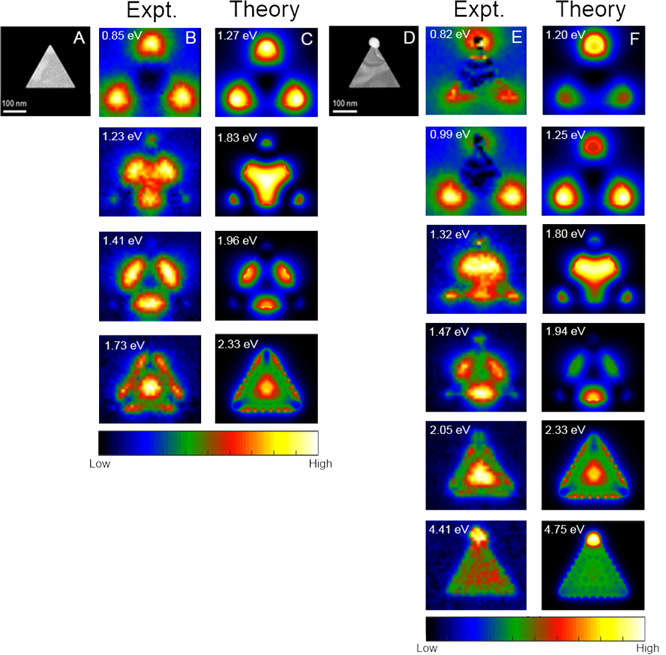
\includegraphics{prisms_mode_maps_tip.png}
\caption{(A-C) Experiments and simulations for a bare Au nanoprism, 209 nm edge length and 10 nm in thickness, supported on a Si3N4 membrane. (A) HAADF; (B) Experimentally measured EEL maps for loss-energies representing corner, edge, and facial plasmon modes; (C) Simulated EEL maps. (D-F) Experiments and simulations for a Au nanoprism, 209 nm edge length and 10 nm in thickness, decorated with a 40 nm diameter Pt nanoparticle supported on a Si3N4 membrane. (D) HAADF; (E) Experimentally measured EEL maps for loss-energies representing corner, edge, facial, and Pt plasmon modes; (F) Simulated EEL maps. Note the splitting of the plasmon modes in the vicinity of the Pt particle (0.85 eV) and the mode mixing induced by the Pt particle at higher loss-energies. Experimental and calculated loss- energies for each mode differ as simulations are calculated in vacuum.}
\label{modes_tip}
\end{figure}

\begin{figure}
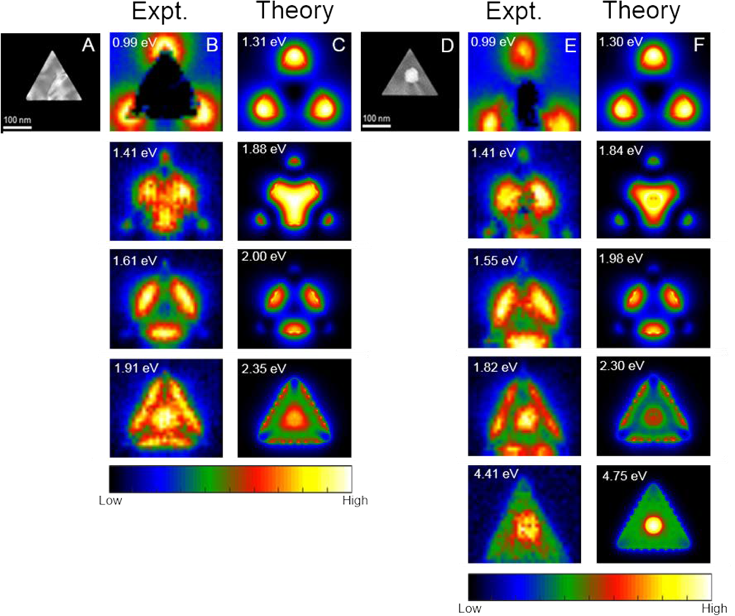
\includegraphics{prisms_mode_maps_center.png}
\caption{(A-C) Experiments and simulations for a bare Au nanoprism, 195 nm edge length and 10 nm in thickness, supported on a Si3N4 membrane. (A) HAADF; (B) Experimentally measure EEL maps for loss-energies representing corner, edge, and facial plasmon modes; (C) Simulated EEL maps. (D-F) Experiments and simulations for a Au nanoprism, 198 nm edge length and 10 nm in thickness, decorated with a 40 nm diameter Pt nanoparticle supported on a Si3N4 membrane. (D) HAADF; (E) Experimentally measure EEL maps for loss-energies representing corner, edge, facial, and Pt plasmon modes; (F) Simulated EEL maps. Note that the low-energy mode structure is conserved between the decorated and undecorated particles due to the three-fold symmetry when Pt is at the center of the prism. Experimental and calculated loss energies for each mode differ as simulations are calculated in vacuum.}
\label{modes_center}
\end{figure}

Figures 1b and 2b show that the plasmon modes of the bare prisms evolve from dipoles localized to the corners, through those on the edges, and finally into multipolar modes as a function of increasing energy, which is in excellent agreement with previous EELS studies of plasmonic nanoprisms.(35, 36) Interestingly, a comparison of the mode maps resulting from decorated and undecorated prisms (Figure 1b,e) shows minimal changes to the mode structure upon addition of the Pt particle. The most notable difference is seen in the splitting of the dipolar mode of the bare Au nanoprism, where the presence of the Pt particle breaks the degeneracy of the dipole mode (vide infra) (Figure 1b,e). Figure 2b,e illustrates that the structure of the higher-energy modes is not strongly dependent on the Pt particle location, as the EEL maps in Figures 1b,e and 2b,e are similar. Lastly, we are able to experimentally map the LSPR of the Pt decoration at a higher energy than the modes of the nanoprism (Figures 1e and 2e).

Boundary element method calculations(37) (Figures 1c,f and 2c,f) capture the complex mode structure of these mixed-metal systems and agree well with the experimental measurements (Figures 1be and 2b,e). While there are quantitative differences in specific plasmon resonance energies between simulation and experiment due to substrate effects, we can leverage the qualitative agreement in the equivalent mode identity to explore the perturbative effects of Pt on the well-understood LSPR modes(38) of Au nanoprisms with plasmon hybridization theory. Previous work(39, 40) has shown that a basis set composed of corner-localized dipoles is sufficient to interpret the low-energy plasmon mode structure of the Au+Pt system. Therefore, we create a model composed of dipoles located on the corners of a triangular prism.(41, 42) Each corner is represented by a disk with two in-plane, orthogonal, dipole plasmons. These single-disk dipoles can be rigorously mapped onto a set of mechanical oscillators and mutually hybridized by diagonalizing the Hamiltonian(43)
\begin{equation}
H = \frac{1}{2}\sum_{i}\hbar\omega_{\textrm{sp}^i}[\textbf{P}_i^2 + \textbf{Q}_i^2] - \frac{1}{2}\sum_{i \neq j}\hbar(\omega_{\textrm{sp}}^i\omega_{\textrm{sp}}^j)^{1/2}g_{ij}(r_{ij})[3(\textbf{Q}_i\cdot\hat{\textbf{n}}_{ij}\hat{\textbf{n}}_{ij}\cdot\textbf{Q}_j)-\textbf{Q}_i\cdot\textbf{Q}_j],
\label{prism_hammy}
\end{equation}
with distance-dependent coupling constants $g_{ij}(r_{ij}) = 3/[r_{ij}^3(\varepsilon_{\infty} + 2)]$ where $i$ and $j$ ($i, j = 1–6$) indicate the identity of each plasmon (location and orientation); $\textbf{Q}_i$ is the coordinate of the $i$th oscillator with conjugate momentum $\textbf{P}_i$; $\omega_{\textrm{sp}}^i$ is its surface plasmon resonance frequency; $r_{ij}$ are the dimensionless distances between the $i$th and $j$th disks relative to their diameters; and $\hat{\textbf{n}}_{ij}$ is the corresponding unit vector connecting them.
In analogy to the mixing of carbon p-orbitals in benzene, the mixing of these six single-disk modes result in six hybridized modes: the lowest-energy mode having no nodes; the second lowest being two degenerate, single-node modes (dipole modes); the third lowest being two degenerate, double-node modes; and the highest-energy mode having three nodes. To produce a quantitative fit to the experimental and simulated data, we choose the resonance frequencies of the disk plasmons so that the resulting dipole plasmon resonance of the Au prism produces the experimentally measured resonance energy (∼1.00 eV).
With this simple model in hand, we are now able to explore the perturbing effects of a Pt particle. Simulation using experimentally derived dielectric data(24) predicts the plasmon resonance of the Pt particle to be near 5.00 eV, which is at a significantly higher energy than the LSPR modes of the Au nanoprism. We introduce the Pt particle to the system as a disk with two degenerate, in-plane, orthogonal dipoles with resonance energies of 5.00 eV, as dictated by experiment on single Pt particles. The plasmon resonances of the collective system are explored with the same hybridization method as before.
Figure 3 displays the hybridization model describing the interaction between the Au nanoprism dipole modes and the Pt dipole modes together with corresponding experimental EEL maps that illustrate the effect of the Pt on the Au nanoprism. Depositing the Pt particle at the center of the nanoprism gives the system 3-fold symmetry and, in turn, does not significantly perturb the LSPR modes of the nanoprism. The mode mixing does cause a small, equal net lowering of the prism-localized collective dipole modes and a small, equal net raising of the Pt-localized collective dipole modes. As the Pt particle is moved toward a corner, however, the system’s dipole modes begin to split. When the prism and the Pt-localized dipole modes are oriented in the same direction, they couple more strongly than when the dipoles are oriented antiparallel; therefore, the former is lower in energy, as expected.(41) The model further shows that this splitting is maximal when the Pt particle is as close to the corner as possible, which is consistent with experimental results.

\begin{figure}
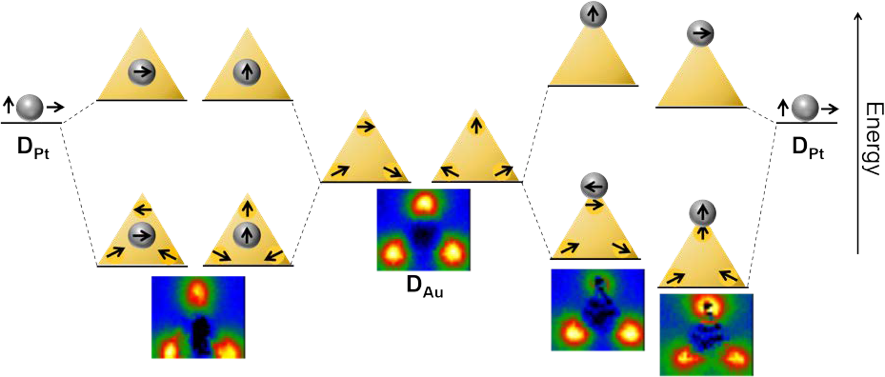
\includegraphics{prisms_theory.png}
\caption{Dipole oscillator model of the mode mixing between the Au prism dipoles (DAu) and the Pt sphere dipoles (DPt). The anti-bonding Pt-centered modes are blue-shifted far from the prism modes upon mixing; whereas, the bonding modes remain centered on the nanoprism and depend much more noticeably upon the placement of the Pt particle. Placing the Pt particle in the center of the Au prism (left) causes a net lowering of the dipole modes but no splitting. The lack of splitting is observed experimentally in the 0.99 eV mode map. Placement of the Pt particle at the tip (right) induces splitting between the formerly degenerate dipolar prism modes, as observed in the experimentally derived mode maps at 0.99 eV and 0.82 eV loss-energies.}
\label{mo_diagram}
\end{figure}

Figure 4a compares the simulated EEL spectra of a 209 nm pure Au nanoprism (black), a 209 nm Au+Pt nanoprism (red) where the 40 nm diameter Pt decoration is at the tip of the nanoprism, and an aloof EEL spectrum of a 40 nm diameter Pt sphere (purple). The Au nanoprism is plasmonically active at energies between 0.90 and 2.40 eV, whereas the Pt sphere is active at a much higher energy (∼5.00 eV). Because of the spectral mismatch in plasmon resonance energies of Au and Pt, these metals are not expected to significantly hybridize and resonance energy transfer is unfavorable. The Pt decoration, therefore, simply acts as part of the dielectric environment, and the plasmons of the prism couple to their images in the Pt particle and vice versa. This image effect is identical for all of the Au and Pt dipole plasmons in the center-decorated system. However, in the tip-decorated system, the nanoprism dipole that is aligned with the Pt dipole couples more strongly to its image than the other orthogonal dipole and is shifted to lower energy.

\begin{figure}
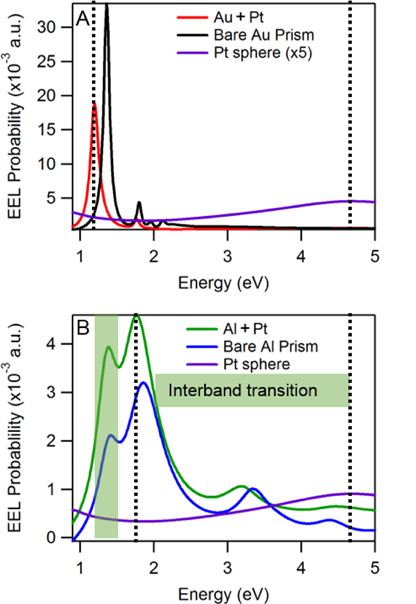
\includegraphics{prisms_EELS_simulation.png}
\caption{Comparison of the calculated EEL spectra at the tip of (A) a 209 nm pure Au nanoprism (black trace), a 209 nm Au+Pt nanoprism (red trace), and a 40 nm diameter Pt sphere (purple trace); (B) a 209 nm bare Al nanoprism (blue trace), a 209 nm Al+Pt nanoprism (green trace), and a 40 nm diameter Pt sphere (purple trace). The interband transition of the Al is centered at 1.40 eV (green box). For each decorated system, the Pt particle is 40 nm in diameter and located at the tip of the nanoprism. Note the slight shifting (~0.15 eV) and broader line- width (FWHM increases by 0.30 eV) in the Al+Pt at ~3.20 eV. This broadening indicates LSPR hybridization between the two metals; whereas, in the Au+Pt system there is a shift of 0.03 eV and a small change in the line-width (FWHM increases by 0.005 eV) at ~1.80 eV. The black dotted lines at 1.20, 1.75, and 4.75 eV correspond to the LSPR of Au+Pt, Al+Pt, and Pt, respectively.}
\label{prisms_EELS_sim}
\end{figure}

The framework presented here, while showing that the Au and Pt plasmons remain mostly uncoupled, does offer insight into the construction of systems with highly coupled plasmon modes for plasmon-mediated catalysis. Consequently, we study Al prisms(44, 45) decorated with Pt because the Al plasmons lie at energies higher than those of Au.(46) Figure 4b compares simulated EEL spectra for a 209 nm Al nanoprism (blue), a 209 nm Al+Pt nanoprism (green) with a 40 nm Pt tip decoration, and a 40 nm diameter Pt sphere (purple). The spectrum of the 3.20 eV peak in the Al+Pt system is broadened by 0.31 eV, determined from the full width at half-maximum (fwhm), with respect to the higher-energy Al prism-localized LSPR modes (∼3.20 eV), suggesting stronger hybridization with the Pt dipole plasmons than in the Au+Pt system. Both Pt and Al have low-energy interband transitions (0.90 and 1.40 eV, respectively) that are not expected to hybridize because of their poor spectral overlap.(47)
To further explore the properties of Al coupled with Pt, Figures 5 and 6 compare the magnitude of the electron-beam-induced electric near-fields of the Al+Pt and Au+Pt systems at three loss-energies: 1.20, 1.75, and 4.75 eV, as indicated in Figure 4 (dotted, vertical lines). Qualitatively similar electric near-fields would arise in response to linearly polarized plane-wave excitation because of the common polarization it shares with the field of the electron at the indicated beam position (x). The field maps reveal that at the energy of the prism-localized dipole mode (Figure 5a,b) and the energy of the Pt-localized dipole mode (Figure 5c,d), the fields around the Pt particles are similar in magnitude. This is reinforced in Figure 5e,f, which present the electric field magnitudes computed along lines (white) bisecting the Pt particle and clearly show electric fields of similar magnitudes for both systems.

\begin{figure}
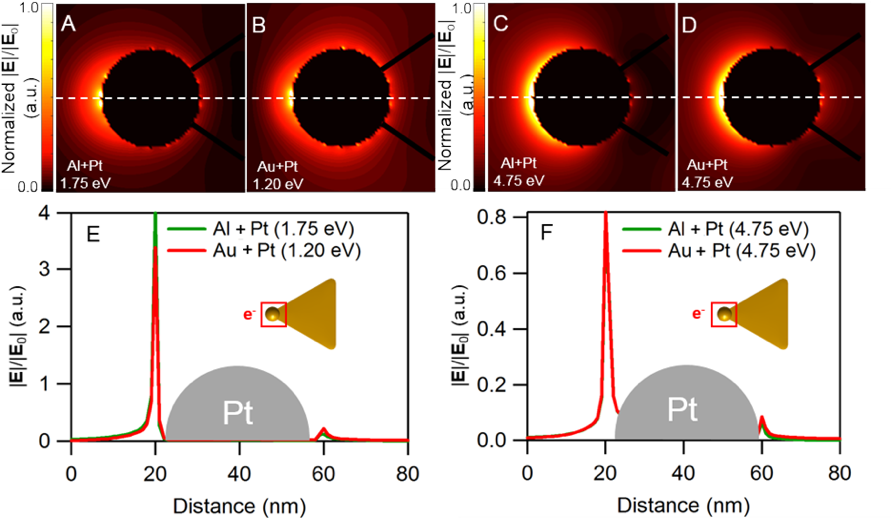
\includegraphics{prisms_field_calculations.png}
\caption{Electric field maps, resulting from electron beam excitation (e-), computed in the plane bisecting the Pt particle and above the prism at the resonance frequencies of the prism dipole plasmons for Al+Pt (A, 1.75 eV) and Au+Pt (B, 1.20 eV). Electric field maps are computed for the same systems, Al+Pt (C) and Au+Pt (D), at the Pt dipole plasmon. Note that the fields become more diffuse around the tip at the Pt resonance frequency (4.75 eV). The fields along the white dotted line are plotted for the prism dipole resonance of Al+Pt and Au+Pt (E, green and red traces, respectively), and for the Pt dipole resonance in Al+Pt and Au+Pt (F, green and red traces, respectively). The gray shapes mark the positon of the sphere. Note that the fields are much larger at the low-energy, hybridized dipoles, but for both systems the fields are comparable in magnitude at similar energies.}
\label{field_top}
\end{figure}

\begin{figure}
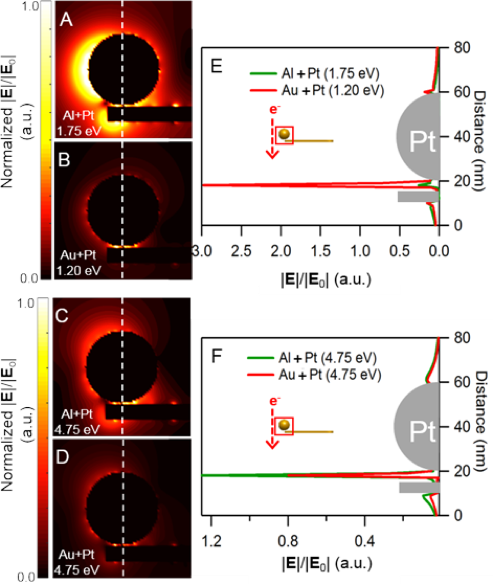
\includegraphics{prisms_fields_2.png}
\caption{Electric field maps, resulting from electron beam excitation (e-), computed in the plane bisecting both the Pt particle and the prism at the resonance frequencies of the dipole plasmons for Al+Pt (A, 1.75 eV) and Au+Pt (B, 1.20 eV) and the dipole plasmon of the Pt (4.75 eV) particle in Al+Pt (C) and Au+Pt (D). Note that the fields in the junction consistently drown out the fields around the particle, except at the dipole of the Al+Pt.
Additionally, along the white dotted line, the fields are plotted for the dipole resonance of Al+Pt and Au+Pt (E, green and red traces, respectively), and for the dipole resonance of the Pt in Al+Pt and Au+Pt (F, green and red traces, respectively). The gray shapes mark the positions of the prism and sphere. Interestingly, the low-energy dipole mode of Au+Pt has a large field in the junction, likely due to Au being a good plasmonic antenna, but the junction field is higher in Al+Pt at the dipole resonance of the Pt. This may be a signature of energy transfer in Al+Pt at these energies.}
\label{field_side}
\end{figure}

Turning to the field magnitude in the junction at the energy of the prism-localized dipoles (Figure 6a,b), we see that the field is much larger in the Au+Pt junction than in the Al+Pt junction. This means that the junction field in the Au+Pt systems is dominated by the response of the Au nanoprism. Conversely, at the energy of the Pt-localized dipole (Figure 6c,d), the junction field in the Al+Pt system is much larger than that of Au+Pt. These observations are again reinforced by the electric field magnitudes presented in Figure 6e,f, which are computed along lines (white) running through the junction. Taken together, Figures 4–6 indicate a relationship between EEL probability and the strength of the near electric fields surrounding the mixed-metal systems observed in this Letter. These junction fields show that the high-energy modes of the nanoprism are more effectively coupled to the Pt dipole plasmon in Al+Pt than in Au+Pt; therefore, a greater capacity for plasmon-mediated chemical catalysis is predicted in the Al+Pt system. Utilizing the electric near-field simulations and data obtained through experiment and calculations, we show that these plasmonic-catalytic metal systems should drive plasmon-assisted reactions.
This work shows through electrodynamics simulations and experimental EELS the extent to which Au nanoprisms decorated with Pt deposits can transfer energy. EELS demonstrates that Pt changes the mode structure of the Au nanoprism, especially depending on the location of the Pt. Even though we show weak coupling between Au and Pt, we determine stronger coupling can be observed in systems where the LSPRs spectrally overlap. In a system such as Al+Pt, the LSPRs of Al and Pt exhibit more spectral overlap because both metals support LSPRs in the ultraviolet regime.

\section{Methods}

In a typical synthesis, fully described in the Supporting Information, reduction of H2PtCl6 on the surface of AUT (11-amino-1-undecanethiol hydrochloride)-conjugated nanoprisms resulted in the growth of approximately 1–3 Pt nanoparticles (average diameter of 30 ± 5 nm) per Au nanoprism substrate. Using high-resolution transmission electron microscopy (HRTEM), it was found that the Pt nanoparticles had a dendritic morphology (SI Figure 3). Interestingly, nucleation of the Pt nanoparticles occurred predominantly on the edges and vertices of the Au nanoprisms, likely due to the higher concentration of defects in the self-assembled monolayer at these sites.(48)
Post-synthesis, Au nanoprisms and Pt-decorated Au nanoprisms were sonicated for 5 min and 2.5 μL of each NP solution was drop-cast onto two separate (S)TEM compatible Si3N4 substrates with 30 nm thick membrane acquired from SPI Supplies. These samples were covered to eliminate contamination and left to air-dry for 3 h prior to EELS acquisition. EEL spectra were acquired in a monochromated Carl Zeiss Libra 200MC (S)TEM operated with an accelerating voltage of 200 kV. Each spectrum acquisition was executed with a collection semiangle of 12 mrad, a convergence semiangle of 9 mrad, and a dispersion of 29 meV per channel. Energy resolution, defined as the full width at half-maximum of the zero-loss peak, for each acquisition is 150 meV with the electron beam probing only the Si3N4 membrane. For each nanoprism, EEL spectrum images responsible for producing LSPR mode maps were collected by defining a region of interest (ROI) around the particle with dimensions 34 × 29 pixels, where 1 pixel is ∼3.3 × 3.3 nm2.
Experimentally obtained EELS mode maps are analyzed using Gatan Digital Micrograph software. Experimental EEL LSPR mode maps (Figures 1b,e and 2b,e) are generated by removing the background using the reflected-tail model and normalized to the zero-loss peak. LSPR mode maps were prepared by plotting spectral intensities from energy slices selected from peak maxima of the single-point spectra from the top corner, edge, bottom corner, face, and center of the Pt decoration to fully represent the LSPR modes of the bare Au nanoprism and the Pt-decorated Au nanoprism system.
For simulations, we applied the Metal Nanoparticle Boundary Element Method (MNPBEM) software.(37) MNPBEM represents nanoparticles as surfaces and discretizes each particle into a chosen number of surface elements. Maxwell’s equations are solved at each of these so-called boundary elements in order to calculate the nanoparticle’s optical properties. EELS simulations were performed on Au and Al nanoprisms with edge lengths of 195 and 209 nm and Au+Pt and Al+Pt nanoprism systems with prism edge lengths of 198 and 209 nm and decorated with Pt spheres of diameter 40 nm at the center and tip, respectively. Each system was simulated with no substrate. These simulations used tabulated dielectric data from Johnson and Christy(49) and Rakic et al.(50) Spectra were acquired at beam positions located at all three corners and edges of each system. Additionally, EEL maps were generated at each of the relevant energy windows. Finally, MNPBEM was used to generate maps of the electric field magnitude around the systems using the electron beam as a source.

% ========== Chapter 3
 
\chapter{Paper 2: Magnetic Plasmons}
 
 
% ========== CHapter 4

\chapter{Conclusion and Future Work}

Conclusion conclusion conclusion

\section{Future Work: Photon-Assisted Electron Spectroscopies}

\subsection{First- and Second-order Fermi's Golden Rule}

Fermi's Golden Rule in first order takes the form
\begin{equation}
\Gamma_{fi} = \frac{2\pi}{\hbar^2}|\langle f |H_{\textrm{int}}| i \rangle |^2 \delta(\omega_f - \omega_i).
\label{FGR_1}
\end{equation}
Here, $\Gamma_{fi}$ is rate at which the system moves from state $i$ to state $f$, $H_{\textrm{int}}$ is the interaction Hamiltonian, and the delta function enforces conservation of energy. In a system with only one perturbation or interaction, computation of the transition rate mediated by that perturbation is straightforward. However, we are interested in a system under the influence of multiple perturbations, specifically a MNP being probed both by light and by a passing electron. THe choice of Fock states matters, but for now we leave them unspecified. Allowing $H_{\textrm{int}} = H_1 + H_2$, Eq. \ref{FGR_1} becomes
\begin{equation}
\begin{aligned}
\Gamma_{fi} &= \frac{2\pi}{\hbar^2}|\langle f |H_1 + H_2| i \rangle |^2 \delta(\omega_f - \omega_i)\\
&= \frac{2\pi}{\hbar}\left[|\langle f |H_1| i \rangle + \langle f |H_2| i \rangle |^2\right] \delta(\omega_f - \omega_i)\\
& = \frac{2\pi}{\hbar}\left[|\langle f|H_1|i \rangle|^2 + |\langle f|H_2|i \rangle|^2 + \langle f|H_1|i \rangle \langle i|H_2|f \rangle + \langle f|H_2|i \rangle \langle i|H_1|f \rangle\right]\delta(\omega_f - \omega_i)
\label{FGR_1_expanded}
\end{aligned}
\end{equation}
Of course, $H_1$ and $H_2$ correspond to two different transitions to two different final Fock states, i.e., the third and fourth terms of Eq. \ref{FGR_1_exapnded} are necessarily zero. The two non-zero rates are mediated by $H_1$ and $H_2$ separately. If $H_1 = H_\textrm{el-pl}$ and $H_2 = H_{\textrm{ph-pl}}$, then the first rate is the EELS rate and the second rate is the absorption rate.

Fermi's Golden Rule for second order transitions looks similar to that for first order transitions:
\begin{equation}
\Gamma_{fi} = \frac{2\pi}{\hbar^4}\left|\sum_{m}\frac{\langle f |H_{\textrm{int}}| m \rangle \langle m |H_{\textrm{int}}| i \rangle }{\omega_f-\omega_i}\right|^2 \delta(\omega_f - \omega_i).
\label{FGR_2}
\end{equation}
Again the Hamiltonian has two terms, $H_{\textrm{int}} = H_1 + H_2$. Wrapping the prefactor, denominator, and delta function together into $A$ to focus on the matrix elements, the rate becomes
\begin{equation}
\begin{aligned}
\Gamma_{fi} &= A|\langle f |H_1 + H_2| m \rangle \langle m |H_1 + H_2| i \rangle|^2\\
&= A|(\langle f |H_1| m \rangle + \langle f |H_2| m \rangle) (\langle m |H_1| i \rangle + \langle m |H_2| i \rangle)|^2\\
&= A(|\langle f |H_1| m \rangle \langle m |H_1| i \rangle|^2 + |\langle f |H_2| m \rangle \langle m |H_2| i \rangle|^2\\
&+ |\langle f |H_1| m \rangle \langle m |H_2| i \rangle|^2 + |\langle f |H_2| m \rangle \langle m |H_1| i \rangle|)^2
\label{FGR_2_2}
\end{aligned}
\end{equation}
For the same reasons as in the discussion of the first order rates, the cross-terms not shown are equal to zero, because $H_1$ and $H_2$ correspond to different transitions with different intermediate and final states. If we now let $H_1 = H_\textrm{el-pl}$ and $H_2 = H_{\textrm{ph-pl}}$, the first term is $\Gamma_{\textrm{EELS}}^{(2)}$, the second term is $\Gamma_{\textrm{abs}}^{(2)}$, the third term is $\Gamma_{\textrm{EEGS}}$ or is related to $\Gamma_{\textrm{SEELS}}$, and the final term is $\Gamma_{\textrm{CL}}$.

\subsection{Quantum-Mechanical Description of EELS, EEGS, SEELS, and CL}

\subsection{Classical Description of EELS}

A common way to compute the EELS rate is by calculating the induced field of the plasmon and having it act on the passing electron via [citation needed]
\begin{equation}
\Gamma_{\textrm{EELS}}(\textbf{r},\omega) = \frac{e}{\pi\hbar\omega}\int dt \textrm{Re}\left\{ e^{-\textrm{i}\omega t} \textbf{v} \cdot \textbf{E}_{\textrm{ind}}(\textbf{r},\omega)\right\}.
\label{eels_rate_bem_1}
\end{equation}
Here, $\textbf{v}$ is the velocity of the electron. It will be more convenient to write the EELS rate in terms of the electron electric field and the induced dipole moment of the plasmon. First, the induced field is written in terms of induced potentials
\begin{equation}
\begin{aligned}
\textbf{E}_{\textrm{ind}} &= -\nabla\phi_{\textbf{ind}} - \frac{\dot{\textbf{A}}_{\textrm{ind}}}{c}\\
&= -\nabla\phi_{\textrm{ind}} + \textrm{i}k\textbf{A}_{\textrm{ind}}.
\label{field_induced}
\end{aligned}
\end{equation}
The induced scalar potential $\phi_{\textrm{ind}}$ and vector potential $\textbf{A}_{\textrm{ind}}$ are related to the induced charge and current densities, respectively
\begin{equation}
\begin{aligned}
&\phi(\textbf{x},\omega) = \int d^3x' \frac{e^{\textrm{i}k|\textbf{x}-\textbf{x}'|}}{|\textbf{x}-\textbf{x}'|}\rho(\textbf{x}',\omega)\\
&\textbf{A}(\textbf{x},\omega) = \int d^3x' \frac{e^{\textrm{i}k|\textbf{x}-\textbf{x}'|}}{|\textbf{x}-\textbf{x}'|}\frac{\textbf{J}(\textbf{x}',\omega)}{c}.
\label{potentials}
\end{aligned}
\end{equation}
Defining $t = z/v$, $dt = dz/v$, and $q = \omega/v$, and plugging Eq. \ref{potentials} and \ref{field_induced} into Eq. \ref{eels_rate_bem_1}, the EELS rate becomes
\begin{equation}
\Gamma_{\textrm{EELS}} = \frac{e}{v\pi\hbar\omega}\int dz \textrm{Re}\left\{ e^{-\textrm{i}qz} \textbf{v} \cdot \left[\int d^3x' \left(-\nabla\frac{e^{\textrm{i}k|\textbf{x}-\textbf{x}'|}}{|\textbf{x}-\textbf{x}'|}\rho(\textbf{x}',\omega)\right) + \textrm{i}k\left(\frac{e^{\textrm{i}k|\textbf{x}-\textbf{x}'|}}{|\textbf{x}-\textbf{x}'|}\frac{\textbf{J}(\textbf{x}',\omega)}{c}\right)\right]\right\}.
\label{eels_with_potentials}
\end{equation}
Defining the Green's function $e^{\textrm{i}k|\textbf{x}-\textbf{x}'}/|\textbf{x}-\textbf{x}'| = 4\pi G(\textbf{x},\textbf{x}')$ allows us to write down a pseudo-potential $\psi = \int dz e^{-\textrm{i}qz} G(\textbf{x},\textbf{x}')$. Integrating by parts deals with the gradient in Eq. \ref{eels_with_potentials} by moving it to $\psi$ as follows: 
\begin{equation}
\int dz e^{-\textrm{i}qz} \nabla G(\textbf{x},\textbf{x}') = e^{-\textrm{i}qz} G(\textbf{x},\textbf{x}') \hat{\textbf{z}} \Big|_{-\infty}^{\infty} + \textrm{i}q \psi \hat{\textbf{z}}.
\label{psi_integral}
\end{equation}
The first term on the right hand side, the surface term, is zero, so the integral of the gradient of the Green's function is simply $\textrm{i}q\psi$.

Rewriting $G$ in terms of its Fourier transform reveals a route to computing the integral in $z$. Doing so results in a new form for the pseudo-potential
\begin{equation}
\begin{aligned}
\psi &= \int dz e^{-\textrm{i}qz} G(\textbf{x},\textbf{x}')\\ 
&= \int dz e^{-\textrm{i}qz} \int \frac{d^3k'}{(2\pi)^3} \frac{4\pi}{k'^2 - k^2} e^{\textrm{i}\textbf{k}'\cdot(\textbf{x}-\textbf{x}')}\\
&= \int \frac{d^3k'}{(2\pi)^3} \frac{4\pi}{k'^2 - k^2} e^{\textrm{i}[k'_x(x-x')+k'_y(y-y')-k'_zz']} \int dz e^{-\textrm{i}(q-k'_z)z}\\
&= \int \frac{d^3k'}{(2\pi)^3} \frac{4\pi}{k'^2 - k^2} e^{\textrm{i}[k'_x(x-x')+k'_y(y-y')-k'_zz']} 2\pi\delta(q-k'_z)\\
&= \int \frac{d^3k'}{(2\pi)^3} \frac{4\pi}{k'^2 - k^2} e^{\textrm{i}\textbf{k}'\cdot(\textbf{x}_{\perp}-\textbf{x}')} 2\pi v \delta(\omega-\textbf{v}\cdot\textbf{k}').
\label{psi_k_space}
\end{aligned}
\end{equation}
We will see that through this definition of $\psi$ we can construct the electron's electric field. However, we rewrite Eq. \ref{eels_with_potential} in terms of $\psi$
\begin{equation}
\Gamma_{\textrm{EELS}} = \frac{4e}{v\hbar\omega}\textbf{v}\cdot\textrm{Re}\int d^3x' \psi(\textbf{x}_{\perp},\textbf{x}',\omega) \left[-\textrm{i}q\rho(\textbf{x}',\omega)\hat{\textbf{z}} + \textrm{i}k\frac{\textbf{J}(\textbf{x}',\omega)}{c}\right],
\label{eels_with_psi}
\end{equation}
and turn our attention to the induced charge and current densities. The densities are defined by an induced dipole moment, $\textbf{d}_{\textrm{ind}}$ as follows:
\begin{equation}
\begin{aligned}
\rho(\textbf{x}',\omega) = \textbf{d}\cdot\nabla_{r}\delta(\textbf{x}'-\textbf{r})&\\
\textbf{J} = \textrm{i}\omega\textbf{d}\delta(\textbf{x}'-\textbf{r})&.
\label{densities}
\end{aligned}
\end{equation} 
Plugging Eq. \ref{densities} into Eq. \ref{eels_with_psi} gives the EELS rate
\begin{equation}
\Gamma_{\textrm{EELS}} = \frac{4e}{v\hbar\omega}\textbf{v}\cdot\textrm{Re}\int d^3x' \psi(\textbf{x}_{\perp},\textbf{x}',\omega) \left[-\textrm{i}q \textbf{d}\cdot\nabla_{r}\delta(\textbf{x}'-\textbf{r})\hat{\textbf{z}} + \textrm{i}k\frac{\textrm{i}\omega\textbf{d}\delta(\textbf{x}'-\textbf{r})}{c}\right]
\label{eels_with_densities}
\end{equation}

A useful mathematical identity allows $\psi\textbf{d}\cdot\nabla_r\delta(\textbf{x}'-\textbf{r}) = \textbf{d}\cdot(\nabla_r\psi)\delta(\textbf{x}'-\textbf{r})$, and the integral over both delta functions makes the replacement $\textbf{x}' \rightarrow \textbf{r}$. In addition, taking the gradient of $\psi$ results in $\nabla_r\psi(\textbf{x}_{\perp},\textbf{r},\omega) = -\textrm{i}\textbf{k}'\psi(\textbf{x}_{\perp},\textbf{r},\omega)$. The EELS rate becomes
\begin{equation}
\Gamma_{\textrm{EELS}} = \frac{4e}{v\hbar\omega}\textbf{v}\cdot \textrm{Re}\psi(\textbf{x}_{\perp},\textbf{r},\omega) \left[(\textrm{i}q)(\textrm{i}\textbf{k}') \cdot \textbf{d}\hat{\textbf{z}} - (\textrm{i}k)(\textrm{i}k')\textbf{d}\right]
\end{equation}
The electron has momentum only in the z-direction, so $q\hat{\textbf{z}} = \textbf{q}$. Using this definition and writing out $\psi$ in full results in the following form for the EELS rate.
\begin{equation}
\begin{aligned}
\Gamma_{\textrm{EELS}} &= \frac{4e}{v\hbar\omega}\textbf{v}\cdot \textrm{Re}\int \frac{d^3k'}{(2\pi)^3} \frac{4\pi}{k'^2 - k^2} e^{\textrm{i}\textbf{k}'\cdot(\textbf{x}_{\perp}-\textbf{r})} 2\pi v \delta(\omega-\textbf{v}\cdot\textbf{k}') \left[(\textrm{i}\textbf{q})(\textrm{i}\textbf{k}') \cdot \textbf{d} - (\textrm{i}k)(\textrm{i}k)\textbf{d}\right]\\
&= \frac{4\textrm{i}e}{\pi\hbar} \textrm{Im}\int d^3q \frac{\textbf{q} - k\textbf{v}/c}{q^2 - k^2} \cdot \textbf{d} \delta(\omega - \textbf{v} \cdot \textbf{q})\\
&= \frac{4}{\hbar}\textrm{Im}\left\{ \textbf{E}_{\textrm{el}} \cdot \textbf{d}_{\textrm{ind}}\right\}.
\end{aligned}
\end{equation}
Here, since $k$' is an integration variable, it has been rewritten as $q$ and the definition of the electron's electric field from Ref. [whatever] has been used to replace $\psi$. So, the common implementation of the EELS rate using the induced electric fields and electron velocity is entirely consistent with the method of using the induced dipole moment and electron electric field.
\section{What I have coded}

I have coded the EELS rate, except I add the surface charges (equivalently, the fields) from both a planewave source and an e-beam source. The EELS rate

\begin{equation}
\Gamma_{\textrm{EELS}} = \frac{1}{\pi\hbar\omega} \int dt \textrm{Re}\{e^{-\textrm{i}\omega t} \dot{\textbf{d}}_{\textrm{ind}} \cdot \textbf{E}_{\textrm{el}} \} .
\label{eels_1}
\end{equation}

Assuming that $\textbf{d}_{\textrm{ind}}$ is induced by both light and the electron and that it oscillates at frequency $\omega$ I rewrite the EELS rate as

\begin{equation}
\Gamma_{\textrm{EELS}} = \frac{1}{\pi\hbar\omega} \int dt \textrm{Re}\{e^{-\textrm{i}\omega t} \frac{d}{dt}[\alpha(\textbf{E}_\textrm{el} + \textbf{E}_{\textrm{ph}})] \cdot \textbf{E}_{\textrm{el}} \}.
\label{eels_2}
\end{equation}

That time derivative is likely not trivial (but perhaps in the case of white light it kicks down a factor of $\textrm{i}\omega$ if the dipole oscillates at frequency $\omega$). However, the above equation shows that adding a light source to an EELS experiment leads to an observable that is proportional to $(\textbf{E}_{\textrm{el}}\cdot\textbf{E}_{\textrm{el}})+(\textbf{E}_{\textrm{el}}\cdot\textbf{E}_{\textrm{ph}})$. The literature claims this is SEELS (or PAEELS, or PINEM).

%
% ==========   Bibliography
%
\nocite{*}   % include everything in the uwthesis.bib file
\bibliographystyle{plain}
\bibliography{uwthesis}
%
% ==========   Appendices
%
\appendix
\raggedbottom\sloppy
 
% ========== Appendix A
\chapter{Supporting Information: Imaging Energy Transfer in Pt-Decorated Au Nanoprisms via Electron Energy-Loss Spectroscopy}

\section{General Materials and Methods}

General materials and methods. Hexadecyltrimethylammonium bromide (CTAB, 99\%), chloroplatinic acid (H2PtCl6, 8 wt. \% in H2O) hydrogen tetrachloroaurate trihydrate (HAuCl4•3H2O, 99.999\%), L-ascorbic acid (99\%), sodium borohydride (NaBH4, 99.99\%), sodium hydroxide (99.99\%), sodium iodide (NaI, 99.999\%), and trisodium citrate (99\%) were obtained from Sigma Aldrich and used as received. 11-amino-1-undecanethiol hydrochloride (AUT, 99.2\%) was purchased from Dojindo (Rockville, MD) and used as received. NANOpure™ water Thermo Scientific, > 18.2 MΩ•cm) was used for all washing, synthesis, and purification protocols as well as in the preparation of all solutions. All stock solutions were aqueous and prepared fresh before each reaction, unless otherwise noted. All glassware was washed with aqua regia (3:1 ratio of concentrated HCl and HNO3 by volume) and rinsed thoroughly with water.

\section{Au Nanoprism Synthesis}

Au nanoprisms were synthesized according to previous protocols. (1, 2) Two hours after Au nanoparticle seeds were added to the nanoprism growth solution, the reaction mixture was heated in a H2O bath to 37 °C for 1 minute to dissolve any CTAB that may have recrystallized during the growth period (this crystallized CTAB can interfere with nanoprism purification by centrifugation). To separate the nanoprisms from pseudospherical nanoparticle reaction byproducts, 90 mL of the reaction mixture was divided into 15 mL conical tubes and
centrifuged at 820 rcf for 15 minutes (Eppendorf centrifuge 5804 with swing bucket rotor A-4-44). The supernatant and pellet were both extracted and the nanoprism thin film was resuspended in 1.0 mL of H2O by vortexing for 5 seconds. To remove additional CTAB and excess reagents, this mixture was transferred to 1.5 mL centrifuge tubes, and the prisms were then centrifuged using a Spectrum minicentrifuge (SC1006-R) for approximately 5 minutes. After centrifugation, the supernatant was removed and the prisms were resuspended in 1.0 mL of H2O and subsequently combined in a 15 mL conical tube. The concentration of the purified nanoprisms in the nanoprism stock solution was then adjusted to an optical density (O.D.) of 1.0 a.u. at the maximum absorption wavelength (λmax, approximately 1300 nm) by ultraviolet-visible-near infrared (UV-vis-NIR) spectroscopy.

\section{Pt-decorated Au Nanoprism Synthesis}

To 1.0 mL of purified Au nanoprisms (absorbance at λmax = 1.0 a.u.) was added 8.0 μL of 1 mM AUT. The mixture was
vortexed, and the nanoprisms were allowed to rest for 24 hours to allow for thiol conjugation to the nanoparticle surface. After this period, 20 μL of 20 mM ascorbic acid was added, and the nanoparticle solution was vortexed briefly. Next, 20 μL of 2 mM H2PtCl6 was added, the solution was briefly vortexed, and the nanoprisms were allowed to rest for an additional 24 hours to ensure complete reduction of H2PtCl6. 

\section{UV-vis-NIR Spectroscopy}

Nanoprism solutions were analyzed by UV-vis-NIR spectroscopy using a Cary 5000 spectrophotometer (Agilent, Inc.). Baselines were collected using H2O as reference solutions.

\section{Transmission Electron Microscopy (TEM)}

Nanoparticle products were purified by centrifugation using a Spectrum mini-centrifuge (SC1006-R). After removal of the supernatant, the pellet was resuspended in 1.0 mL of H2O and the process was repeated. After subsequent removal of the supernatant, nanoprism products were resuspended in 30 μL of H2O by vortexing and sonicating for approximately 10 seconds. For general TEM imaging, a 5 μL aliquot of each concentrated nanoprism sample was dropcast onto a TEM grid (Ted Pella, Carbon Type A on 300 mesh Cu), allowed to dry under ambient conditions, and stored under vacuum prior to analysis. TEM images were obtained using a JEOL JEM 2100F equipped with a Gatan Imaging Filter (GIF) Tridiem camera and Oxford Inca EDS detector at 200 kV (Nanoscale Fabrication and Characterization Facility, Petersen Institute of Nanoscience and Engineering, University of Pittsburgh), or a Hitachi Environmental TEM at 300 kV (Department of Mechanical Engineering and Materials Science characterization facility, University of Pittsburgh). Images were analyzed using Digital Micrograph v2.10.1282.0 (Gatan, Inc.) and/or ImageJ v 1.47d (National Institutes of Health, USA) software.

\section{Scanning Electron Microscopy (SEM)}

Silicon wafer substrates (University Wafer, ptype, 200 nm thermal oxide (silicon dioxide)) were first cleaned by sonicating in ethanol for 5 min. The substrate was then successively rinsed with ethanol and acetone and dried under a stream of N2(g). Samples were prepared using the same procedure described for TEM analysis. Here, 10 μL of the resulting solution was drop-cast onto the wafer and allowed to dry before imaging on a Raith Dual Beam EBL-SEM at various accelerating voltages.


\end{document}
